%%%%%%%%%%%%%%%%%%%%%%%%%%%%%%%%%%%%%%%%%
% a0poster Portrait Poster
% LaTeX Template
% Version 1.0 (22/06/13)
%
% The a0poster class was created by:
% Gerlinde Kettl and Matthias Weiser (tex@kettl.de)
% 
% This template has been downloaded from:
% http://www.LaTeXTemplates.com
%
% License:
% CC BY-NC-SA 3.0 (http://creativecommons.org/licenses/by-nc-sa/3.0/)
%
%%%%%%%%%%%%%%%%%%%%%%%%%%%%%%%%%%%%%%%%%

%----------------------------------------------------------------------------------------
%	PACKAGES AND OTHER DOCUMENT CONFIGURATIONS
%----------------------------------------------------------------------------------------

\documentclass[a0,portrait]{a0poster}

\usepackage{multicol} % This is so we can have multiple columns of text side-by-side
\columnsep=100pt % This is the amount of white space between the columns in the poster
%\columnseprule=3pt % This is the thickness of the black line between the columns in the poster

\usepackage[svgnames]{xcolor} % Specify colors by their 'svgnames', for a full list of all colors available see here: http://www.latextemplates.com/svgnames-colors

\usepackage{times} % Use the times font
%\usepackage{palatino} % Uncomment to use the Palatino font

\usepackage{graphicx} % Required for including images
\graphicspath{{figures/}} % Location of the graphics files
\usepackage[font={sf,small}, labelfont={bf,sf,small}]{caption} % Required for specifying captions to tables and figures
\usepackage{amsfonts, amsmath, amsthm, amssymb} % For math fonts, symbols and environments
\usepackage{wrapfig} % Allows wrapping text around tables and figures
\usepackage[utf8]{inputenc}
\usepackage{array}
\usepackage{bm}
\usepackage{algorithm}
\usepackage{algorithmic}
\usepackage{sectsty}
\usepackage{tikz}

\providecommand{\subcapfont}{\color{Black} \small}

\providecommand{\norm}[1]{\lVert#1\rVert}
\renewcommand{\Re}[1]{\mathfrak{Re}\lbrace#1\rbrace}
\renewcommand{\Im}[1]{\mathfrak{Im}\lbrace#1\rbrace}

% Algorithmic package, rename "Require/Ensure" into "Input/Output"
\renewcommand{\algorithmicrequire}{\textbf{Input:}}
\renewcommand{\algorithmicensure}{\textbf{Output:}}
\renewcommand{\thealgorithm}{} % needed to remove the numbering of the algorithm

\sectionfont{\color{Orange} \normalfont \sffamily \bfseries}
\subsectionfont{\color{Navy} \normalfont \sffamily \bfseries}

\begin{document}

\sffamily
\normalsize

%----------------------------------------------------------------------------------------
%	POSTER HEADER 
%----------------------------------------------------------------------------------------

% The header is divided into two boxes:
% The first is 75% wide and houses the title, subtitle, names, university/organization and contact information
% The second is 25% wide and houses a logo for your university/organization or a photo of you
% The widths of these boxes can be easily edited to accommodate your content as you see fit

\begin{minipage}[b][12cm][c]{0.65\linewidth}
\sffamily
\veryHuge \color{NavyBlue} \textbf{Finite Dimensional FRI} \color{Black}\\[2cm] % Title
%\Huge\textit{An Exploration of Complexity}\\[2cm] % Subtitle
\huge \textbf{Jon Oñativia$^1$, Yue M. Lu$^2$ and Pier Luigi Dragotti$^1$}\\[1cm]
\large $^1$ Communications and Signal Processing Group (CSP), Imperial College London, UK\\[0.4cm]
\large $^2$ Signals, Information and Networks Group (SING), Harvard University, USA\\[0.4cm]
\end{minipage}
%
\begin{minipage}[b][12cm][t]{0.35\linewidth}
\begin{flushright}
\begin{tabular}{m{16cm} m{8cm}}
\vspace{0pt} \includegraphics[width=14cm]{imperial_logo}  &
\vspace{0pt} 
\includegraphics[width=8cm]{harvard_logo}
\end{tabular}
\end{flushright}
\end{minipage}
% \fbox{
% \begin{minipage}[b][12cm][t]{0.25\linewidth}
% \begin{figure}[h]
% \centering
% \begin{subfigure}{.5\textwidth}
% \fbox{\includegraphics[width=10cm]{imperial_logo}\hspace{2cm}}
% \end{subfigure}
% \begin{subfigure}{.5\textwidth}
% \fbox{
\includegraphics[width=4cm]{harvard_logo}}\\
% \end{subfigure}
% \end{figure}
% \end{minipage}
% }

%\vspace{1cm} % A bit of extra whitespace between the header and poster content

%----------------------------------------------------------------------------------------


\begin{multicols}{2} % This is how many columns your poster will be broken into, a portrait poster is generally split into 2 columns


%----------------------------------------------------------------------------------------
%	ABSTRACT
%----------------------------------------------------------------------------------------

\color{Navy} % Navy color for the abstract

\begin{itemize}

\item Traditional Finite Rate of Innovation (FRI) theory considers the problem of sampling continuous-time
signals.

\item This framework can be naturally extended to the discrete-time case.

\item We present a novel approach based on the traditional FRI sampling scheme that takes 
advantage of the fact that the null space of the problem is finite dimensional.

% \item Perfect reconstruction is guaranteed in the noiseless scenario.

% \item Simulation results in the noisy scenario improves performances in terms of the mean squared
% error (MSE) of the reconstructed signal compared to the canonical FRI algorithms and compressesd
% sensing (CS).

\end{itemize}

%----------------------------------------------------------------------------------------
%	INTRODUCTION
%----------------------------------------------------------------------------------------

%\color{SaddleBrown} % SaddleBrown color for the introduction

\section*{Introduction}

\begin{itemize}

\item FRI sampling theory \cite{vetterli2002,blu2008} has shown that it is possible to sample
and reconstruct classes of non-bandlimited signals.
% Streams of Diracs are the canonical example of FRI signals. They are not bandlimited but 
% are sparse in time and have a finite number of degrees of freedom per unit of time, which is 
% known as the rate of innovation. The final goal of FRI methods is to retrieve the exact 
% location and amplitude of the Diracs from a set of samples. 
\item FRI methods are based on the fact that 
the Fourier transform of a sum of Diracs is given by a sum of exponentials.
The reconstruction is then based on estimating exponentials from a sequence of samples, which is a 
classical problem in spectral estimation \cite{stoica2005}. 

% This framewok can be naturally extended to discrete-time signals. In this case, the sampling 
\item Sampling of discrete-time signals process can be modelled with a matrix multiplication. 
\begin{itemize}
\item The input signal is given by a high dimensional vector with few non-zero elements. 
\item The acquired signal is a vector of lower dimension which is given 
by the product of a fat matrix with the input signal. 
\end{itemize}

% Note that since the acquisition matrix is fat, 
% the dimension of its null space is strictly positive. 

\item The goal is to reconstruct the sparse input vector from the acquired samples. 

\end{itemize}

%----------------------------------------------------------------------------------------
%	Traditional FIR
%----------------------------------------------------------------------------------------

\color{Navy} % DarkSlateGray color for the rest of the content

\section*{Traditional FRI}

\begin{itemize}

\item Let $\bm{x} \in \mathbb{C}^N$ be a discrete time signal formed by a stream of $K$ Diracs:

\begin{equation}
x[n] = \sum_{k=1}^K a_k \, \delta [n - n_k], \qquad n = 0, 1, \ldots, N-1.
\label{eq:sparse_x}
\end{equation}

% \noindent
% where $n_k \in [0,N-1]$ and $a_k \in \mathbb{C} \setminus \{0\}$, for $1 \leq k \leq K$,
% are unknown integer delays and complex valued amplitudes, respectively. 

\item The signal $\bm{x}$ has $2K$ degrees of freedom: 
\begin{itemize}
\item Delays $n_k \in \lbrace 0, 1, \ldots, N-1\rbrace$, for $k=1,\ldots,K$,
\item Amplitudes $a_k \in \mathbb{C} \setminus \{0\}$, for $k=1,\ldots,K$.
\end{itemize}

\item We have access to $M<N$ coefficients of the DFT of $\bm{x}$. 

\item We can express the sampling process in matricial form as follows

\begin{equation}
\bm{y} = \bm{D} \, \bm{x},
\label{eq:under_y}
\end{equation}

\noindent 
where $\bm{y} \in \mathbb{C}^M$ are the available samples and $\bm{D} \in \mathbb{C}^{M \times N}$ 
is a partial Fourier matrix:
$\left(\bm{D}\right)_{m,n} = \exp \left(-j2\pi mn/N\right) / \sqrt{N}$,
with $m=0,\ldots,M-1$ and $n=0,\ldots,N-1$.

\begin{center}\vspace{1cm}
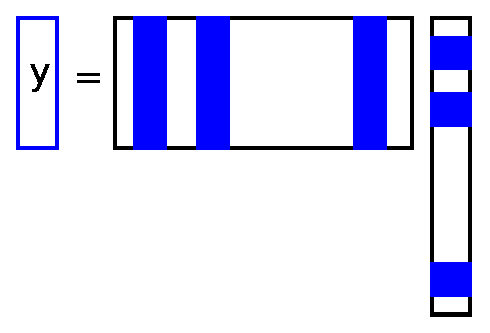
\includegraphics[width=0.4\linewidth]{matrix_mult_2}
\captionof{figure}{Vector $\bm{y}$ is the result of multiplying a fat matrix by a high dimensional sparse vector.}
\end{center}\vspace{1cm}

\item The unitary DFT of $\bm{x}$ 
consists of the sum of $K$ exponentials with frequencies $\omega_k = 2 \pi n_k / N$:

\begin{equation*}
\hat{x}[m] = \tfrac{1}{\sqrt{N}} \sum_{k=1}^K a_k \, e^{-j \omega_k m}, \qquad m = 0, 1, \ldots, N-1.
\end{equation*}

\end{itemize}


\subsection*{Annihilating filter method}

\begin{itemize}

\item Sequence $\hat{x}[m]$ is annihilated by a $K+1$ taps filter $h[m]$: $(\hat{x} * h)[m] = 0$.

\item Filter with zeros at $z=e^{-j \omega_k}$: 
$H(z) = \prod_{k=1}^{K} \left(1-e^{-j \omega_k} \, z^{-1}\right) = 1 + \sum_{m=1}^{K} h[m] \, z^{-m}$.

\item The method is based on finding the $h[m]$ coefficients, and estimating the frequencies
$\omega_k$ from the roots of $H(z)$. Coefficients $h[m]$ are obtained by building a Toeplitz matrix
and establishing the following system:

\begin{equation*}
\normalsize
\begin{bmatrix}
\hat{x}[K] & \hat{x}[K-1] & \ldots & \hat{x}[0]\\
\hat{x}[K+1] & \hat{x}[K] & \ldots & \hat{x}[1]\\
\vdots & \vdots & \ddots & \vdots\\
\hat{x}[2K] & \hat{x}[2K-1] & \ldots & \hat{x}[K]\\
\end{bmatrix}
\cdot
\begin{bmatrix}
1\\ h[1]\\ \vdots\\ h[K]
\end{bmatrix}
= 0
\qquad \Longrightarrow \qquad
\bm{S}\,\bm{h} = \bm{0}.
\end{equation*}

\item We can recover the parameters $a_k$ and $n_k$ from $2K$ samples of $\hat{x}[m]$. The problem is:

\begin{itemize}
\item Nonlinear in $\omega_k.$
\item Linear in $a_k$.
\end{itemize}

\end{itemize}



%----------------------------------------------------------------------------------------
%	New approach
%----------------------------------------------------------------------------------------

\section*{Finite dimensional FRI: new approach}

\begin{itemize}

\item Avoid the root finding step and recover the $K$-sparse vector by solving two linear systems.

\item We can reconstruct $\bm{x}$ from $\bm{y}$ applying the pseudoinverse of $\bm{D}$, up to its null space:

\begin{equation*}
\bm{x} = \bm{D}^H \, \bm{y} + \sum_{l=1}^{L} \beta_l \, \bm{n}_l,
\end{equation*}

\noindent
where $\beta_l$ are unknown coefficients, $L=N-M$ is the size of the null space 
and $\bm{n}_l$ are $L$ vectors that span the 
null space of $\bm{D}$: $\bm{n}_l \in N(\bm{D})$ where 
$N(\bm{D}) = \lbrace \bm{n} \in \mathbb{C}^M \,\vert\, \bm{D} \, \bm{n} = \bm{0} \rbrace$.

\item If we premultiply the previous equation by $\bm{F}_N$ we obtain the 
Fourier transform of $\bm{x}$:

\begin{equation*}
\bm{\hat{x}} 
= \bm{F}_N \, \bm{x} 
= \bm{z} + \sum_{l=1}^{L} \beta_l \, \bm{F}_N \, \bm{n}_l
\qquad 
\overset{\text{Annihilating filter}}{\Longrightarrow}
\qquad
\left( \bm{Z} + \sum_{l=1}^L \beta_l \bm{E}_{M+l} \right) \, \bm{h} = \bm{0}.
\end{equation*}

\item By building the Toeplitz matrices and assuming the annihilating filter $\bm{h}$
is known, we can establish a determined linear system to find the coefficients $\beta_l$:

\begin{equation*}
\begin{bmatrix}
\bm{E}_{M+1} \, \bm{h} & \ldots & \bm{E}_{N} \, \bm{h}
\end{bmatrix}
\,
\begin{bmatrix}
\beta_1\\
\vdots\\
\beta_L
\end{bmatrix}
=
- \bm{Z} \, \bm{h}.
\end{equation*}

\item The annihilating filter can be obtained from $2K$ elements of vector $\bm{y}$.

\item The coefficients $\beta_l$, $l=1,\ldots,L$, correspond to the missing part of $\bm{\hat{x}}$.
We can thus reconstruct $\bm{x}$ by applying the inverse Fourier transform.
\\
\end{itemize}

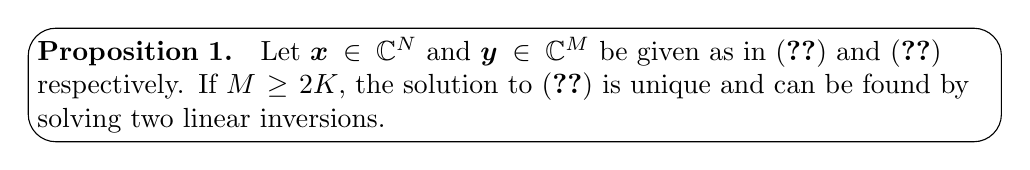
\begin{tikzpicture}
\node[draw=black, rounded corners=10pt, text width=\linewidth] {
\textbf{Proposition 1. }
Let $\bm{x} \in \mathbb{C}^{N}$ and $\bm{y} \in \mathbb{C}^{M}$ be given as in 
\eqref{eq:sparse_x} and \eqref{eq:under_y} respectively. If $M \geq 2K$, the solution to 
\eqref{eq:under_y} is unique and can be found by solving two linear inversions.
};
\end{tikzpicture}

\begin{center}
\begin{tabular}{ccc}
\begin{tabular}{c}
\includegraphics[width=.25\linewidth]{figures/signal_M_256_K_16}\\
\subcapfont (a) Original signal $\bm{x}$
\end{tabular}
&
\begin{tabular}{c}
\includegraphics[width=.45\linewidth]{figures/ft_signal_M_256_N_32_K_16}\\
\subcapfont (b) $\Re{\bm{\hat{x}}}$ and available $M$ samples\\
\includegraphics[width=.45\linewidth]{figures/ft_extrapolate_signal_M_256_N_32_K_16}\\
\subcapfont (c) $\Re{\bm{\hat{x}}}$ and extrapolated coefficients
\end{tabular}
&
\begin{tabular}{c}
\includegraphics[width=.25\linewidth]{figures/signal_reconstr_M_256_N_32_K_16}\\
\subcapfont (d) Reconstructed signal
\end{tabular}
%\normalsize (c) $\Re{\bm{\hat{x}}}$ and available $M$ samples\\
%\includegraphics[width=.45\linewidth]{figures/ft_extrapolate_signal_M_256_N_32_K_16}\\
%\normalsize (d) $\Re{\bm{\hat{x}}}$ and extrapolated coefficients\\
\end{tabular}
\captionof{figure}{$N=256$, $M=32$ and $K=16$. (a) Signal with $K=16$ Diracs. (b) Real part of the 
Fourier coefficients in black and available samples in red. (c) Extrapolated coefficients in red.
(d) Perfect reconstruction of the signal, in red the original signal and in blue the reconstruction.}
\end{center}



%----------------------------------------------------------------------------------------
%	Simulations
%----------------------------------------------------------------------------------------

\section*{Noisy case algorithm and Simulations}

\begin{itemize}
\item In the presence of noise, the reconstruction algorithm is based on 
solving two Total Least Squares problems.
\\
\end{itemize}

\textbf{Input}: Samples $\bm{y}$, number of Diracs $K$

\textbf{Output}: Dirac locations and amplitudes: $\{(n_k, a_k)\}_{k=1}^K$

\begin{enumerate}

\item Denoise samples $\bm{y}$ with Cadzow algorithm
\item Compute the annihilating filter: 
\quad $\bm{h} = \arg \min_{\bm{h}} \; \norm{\bm{Y}^{toe}\,\bm{h}}_2^2$
\item Estimate $\bm{\hat{x}} = [\bm{y} \quad \bm{\beta}]^T$, \\
\qquad where $\bm{\beta} = \arg \min_{\bm{\beta}} \;
\norm{\begin{bmatrix}\bm{Z} \; \bm{h} & \bm{E}_{M+1} \; \bm{h} & \ldots & \bm{E}_{N} \; \bm{h}\end{bmatrix}\,
\begin{bmatrix}1\\\bm{\beta}\end{bmatrix}}_2^2$

\item Esimate locations $n_k$ from $K$ largest local maxima of IDFT$\{\bm{\hat{x}}\}$

\item Estimate amplitudes solving a least squares problem from \eqref{eq:under_y} selecting $K$
columns

\end{enumerate}

% \begin{algorithm}
% \setstretch{1.4}
% \caption{Finite dimensional FRI}
% \algsetup{indent=2em}
% \begin{algorithmic}[1]
% \REQUIRE Samples $\y$, number of Diracs $K$
% \ENSURE  Dirac locations and amplitudes: $\{(n_k, a_k)\}_{k=1}^K$
% \STATE Denoise samples $\y$ with Cadzow algorithm
% \STATE Compute the annihilating filter:
%         $\bm{h} = \arg \min_{\bm{h}} \; \norm{\bm{Y}^{toe}\,\bm{h}}_2^2$
% \STATE Estimate $\bhx = [\y \quad \bm{\beta}]^T$, \\
%         \qquad where $\bm{\beta} = \arg \min_{\bm{\beta}} \;
%         \norm{\begin{bmatrix}\bm{Z} \; \bm{h} & \bm{E}_{M+1} \; \bm{h} & \ldots & \bm{E}_{N} \; \bm{h}\end{bmatrix}\,
%         \begin{bmatrix}1\\\bm{\beta}\end{bmatrix}}_2^2$
% \STATE Esimate locations $n_k$ from $K$ largest local maxima of IDFT$\{\bhx\}$
% \STATE Estimate amplitudes solving the least squares problem\\
%         \qquad $[a_1,\ldots,a_K]^T = \D\left(1:M,[n_1,\ldots,n_K]\right)^\dagger \; \y$
% \end{algorithmic}
% \end{algorithm}

\begin{center}\vspace{1cm}
\includegraphics[width=\linewidth]{simulation_results_dB}
\captionof{figure}{Simulation results showing new finite dimensional FRI approach outperforming
traditional FRI methods (root finding of the annihilating filter or matrix pencil) 
and compressed sensing reconstruction. $N=256$ and $M=64$. Simulations performed at 
different levels of noise (SNR of 5, 10 and 15 dB) and different levels of sparsity $K$ (horizontal axis).
The vertical axis shows the normalized average value of the MSE of the reconstructed
sparse vector compared to the true $\bm{x}$.}
\end{center}\vspace{1cm}



%----------------------------------------------------------------------------------------
%	CONCLUSIONS
%----------------------------------------------------------------------------------------

\section*{Conclusions}

\begin{itemize}

\item Novel method to reconsctruct a finite dimensional sparse vector from partial 
knowledge of its discrete Fourier transform. 

\item In the noiseless scenario, perfect reconstruction is achieved with the critical 
number of samples. 

\item In the noisy case, this method is more stable and outperforms traditional FRI approaches 
and CS because it takes advantage of the fact that the null space of the underdetermined 
system is finite dimensional.

\end{itemize}

%----------------------------------------------------------------------------------------
%	ACKNOWLEDGEMENTS
%----------------------------------------------------------------------------------------

\color{Navy}

\section*{Acknowledgements}

\small
Work supported by the European Research Council starting investigator award Nr. 277800 (RecoSamp).

%----------------------------------------------------------------------------------------
%	REFERENCES
%----------------------------------------------------------------------------------------

\small
\nocite{*} % Print all references regardless of whether they were cited in the poster or not
\bibliographystyle{IEEEtran} % Plain referencing style
\bibliography{sample} % Use the example bibliography file sample.bib

%----------------------------------------------------------------------------------------

\begin{flushright}
\vspace{1.1cm}
\includegraphics[width=8cm]{poster_logo}
\end{flushright}

\end{multicols}




\end{document}
